\documentclass[tikz,border=5pt]{standalone}
\usepackage[utf8]{vietnam}
\usepackage{amsmath,amssymb}
\usepackage{tikz}

\begin{document}
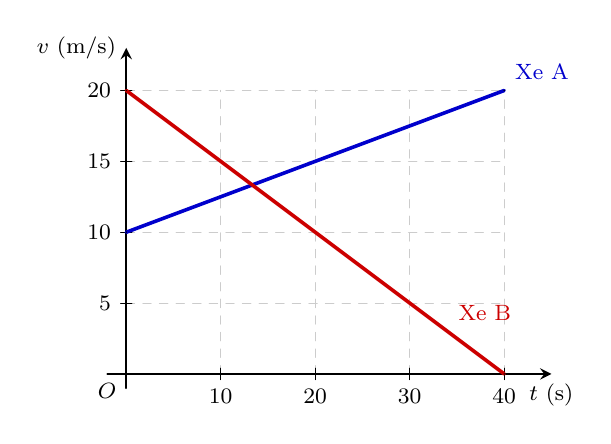
\begin{tikzpicture}[>=stealth, line join=round, line cap=round, font=\footnotesize, xscale=0.12, yscale=0.18]
	% Hệ lưới tọa độ
	\draw[dashed, gray!40, thin] (0, 0) grid[xstep=10, ystep=5] (40, 20);

	% Trục tọa độ
	\draw[->, thick] (-2, 0) -- (45, 0) node[below] {$t\text{ (s)}$};
	\draw[->, thick] (0, -1) -- (0, 23) node[left] {$v\text{ (m/s)}$};
	\node[below left] at (0, 0) {$O$};

	% Vạch chia trục hoành
	\foreach \t in {10, 20, 30, 40} {
		\draw (\t, 0.4) -- (\t, -0.4);
		\node[below] at (\t, -0.4) {$\t$};
	}

	% Vạch chia trục tung
	\foreach \v in {5, 10, 15, 20} {
		\draw (0.6, \v) -- (-0.6, \v);
		\node[left] at (-0.6, \v) {$\v$};
	}

	% Đồ thị Xe A: (0, 10) -> (40, 20)
	\draw[line width=1.3pt, blue!80!black] (0, 10) -- (40, 20) node[above right] {Xe A};

	% Đồ thị Xe B: (0, 20) -> (40, 0)
	\draw[line width=1.3pt, red!80!black] (0, 20) -- (40, 0) node[above right, pos=0.85] {Xe B};

	% Đánh dấu các mốc
	\fill[black] (0, 10) circle (2pt);
	\fill[black] (40, 20) circle (2pt);
	\fill[black] (0, 20) circle (2pt);
	\fill[black] (40, 0) circle (2pt);
\end{tikzpicture}
\end{document}
